%===================================== CHAP 4 =================================

\chapter{Data}
For our analyses we have gathered data on the  S\&P 100 companies. For each company we have collected price data, trading volumes, news article counts, Google Trends data and Wikipedia Pageviews.  
\\\\
We include all companies that were part of S\&P 100 as of July 31, 2017, except Dow DuPont, The Priceline Group, Time Warner inc, Monsanto, and Walgreens Boots Alliance, as they lack Google Trends data. For concept trend, Dow Dupont does not exist in Google Trends, while The Priceline Group changes name during our time period. Walgreens Boots Alliance had null values in the dataset for concept trend, which gives invalid values in our dataset. Time Warner and Mosanto was aquired by AT\&T and Bayer respectively. This leads to missing data. After removing companies with incomplete data we were left with 94 companies and 5983 observations. A complete list of the stock tickers we use in our analyses is given in Appendix \ref{app:company_terms}.
\\\\
To ensure consistency in our dataset and avoid data collection errors, we developed a Python application for collection and transformation of information from the different data sources. The application accepts an input file defining the relevant Wikipedia page, Google Trends terms and stock ticker for each company. It will then automatically generate an Excel file containing all the variables defined below, both in original.


\section{News articles}
News articles are collected from the Thomson Reuters Eikon database where we are able to obtain news articles categorized by the companies they mention. Our dataset covers the time period between July 2017 and September 2018 for both information demand and supply variables, and contains approximately 650 000 news stories. This is about the same time period as \cite{vlastakis} use for the information supply variable in their analyses. The Thomson Reuters Eikon database provides detailed news data and its website provides the following description of the news database:
\\
"Access content from over 400 real-time streaming news sources and financial newswires, over 6,000 near real-time and archived sources, and hundreds of Web sources so that you have the full spectrum of information you need to act first. All regions of the world are covered, including essential emerging markets." (\cite{descriptionThomsonReutersdatabase})
\\\\\
In Thomson Reuters we use Reuters instrument codes (RICs) instead of company names when collecting news articles. RICs allow us to  gather news articles that relates to subsidiaries of a company without doing multiple manual searches for each of them. To extract the news data we wrote a script accessing the Eikon API. It obtains all news articles from the NewsWire and NewsRoom databases, which are tagged as mentioning one of the S\&P 100 companies. For each company we make a weekly count of the number of articles which are tagged with the company RIC.
\\\\
To normalize news data we transform weekly news count, $Nws$, into the Abnormal News Count with the following formula:
\begin{equation}
   \label{abnormal_news} 
   AbnNws_{t} = log(Nws_{t}) - log[Med(Nws_{t-8},...,Nws_{w-1})] 
\end{equation}
\\
where $log(Nws_{t})$ is the logarithm of the news count at week number $t$. $log[Med(Nws_{t-8},...,Nws_{t-1})]$ is the logarithm of the median $Nws$ for the previous 8 weeks in accordance with \cite{engelberg}. $log$ is defined as the natural logarithm in all equations. 
\\\\
\section{Financial data}
Daily financial data for the companies are obtained from the Alpha Vantage API using ticker codes for each company. This includes open, close, high, low, adjusted close, and volume for each ticker. We use weeks starting and ending on Mondays when calculating financial variables. This is to make sure all variables have comparable time periods. As Google Trend uses weeks starting on Sunday and ending on Saturday, Monday is the first available trading day after the Google Trends week ends. 
\subsection*{Return}
We use Equation \eqref{log_return} to calculate the weekly log return:
\begin{equation}
   \label{log_return} 
   R_t = log (C_{t+1}/C_{t}) 
\end{equation}
where $C_{t}$ is the adjusted Monday closing price and $R_{t}$ is the return for week $t$.
\\\\
\subsection*{Trading volume}
\begin{equation}
   \label{abnormal_volume} 
   Volume_{t} = log(RawVolume_{t}) - log[Med(RawVolume_{t-8},...,RawVolume_{t-1})] 
\end{equation}
We use the following equation to calculate the daily Abnormal Trading Volume ($AbnVlm$) for a company: 
\begin{equation}
   \label{abnormal_volume} 
   AbnVlm_{t} = log(Vlm_{t}) - log[Med(Vlm_{t-8},...,Vlm_{t-1})] 
\end{equation}
   where $AbnVlm_t$ is the Abnormal Trading Volume at week $t$. $log(Vlm_{t})$ is the logarithm of the trading volume at week $t$. $log[Med(Vlm_{t-8},...,Vlm_{t-1})]$ is the logarithm of the median $Vlm$ for the previous 8 weeks.
\subsection*{Volatility}
We use the \cite{garman} volatility estimator adjusted for opening jumps as discussed in \cite{molnar_volatility}.
The following formula is used to calculate daily variance:
\begin{equation}
   \label{w_volatility} 
    \sigma^2_{d} = \frac{1}{2}(h_d-l_d)^2-(2log(2)-1)c_d^2+jadj_d^2
\end{equation}
with:
\begin{equation}
\begin{split}
c_{d} = log(close_{d})-log(open_{d}) \\
l_{d} = log(low_{d})-log(open_{d}) \\
h_{d} = log(high_{d})-log(open_{d}) \\
j_{d} = log(open_{d})-log(close_{d-1}) \\
r_{d} = log(close_{d})-log(close_{d-1}) \\
radj_{d} = log(aclose_{d})-log(aclose_{d-1}) \\
jadj_{d} = j_{d} \frac{radj_{d}}{r_{d}} \\
\end{split}
\end{equation}
Weekly variance is calculated as:
\begin{equation}
   \label{w_volatility} 
    \sigma^2_{t} = \sum_{d \in t} \sigma^2_{d} 
\end{equation}
Finally weekly volatility is calculated as:
\begin{equation}
   \label{w_volatility} 
    \sigma_t = \sqrt{\sigma^2_t}
\end{equation}
 where $t$ is week number. $high_{d}$ and $low_{d}$ are the highest and lowest quoted price on the given day. $open_{d}$, $close_{d}$, $aclose_{d}$ are the open, close and adjusted close price on the given day. 

\section{Search volume}\label{sec:search volume}
Search volume data is collected from Google Trends which provides data about Google search volume for keywords or concepts. The search volume data is downloaded directly from the Google Trends page. The index is reported as a value between 0 and 100 for the given time period. The Search Volume Index (hereafter called SVI) values are normalized based on the chosen time interval during download, so the highest value equals 100. The SVI values are not meaningful in themselves, as they can be be manipulated to an arbitrary number by changing the time interval. Therefore, it is necessary to standardize the values. Standardization also makes the index more comparable across companies. We standardize by taking the logarithm of the SVI minus its median in the previous 8 weeks. 
\\\\
We collect 3 different Google Trends SVI's per company:
\\\\
\textit{Ticker trend}
\\
Using each company's stock ticker as a keyword
\\\\
\textit{Search term trend}
\\
We follow the method described in  \cite{vlastakis}. We started by inserting the full company name and all the variations known to us to Google Insights for Search and chose the keyword with the largest search volume.
\\\\
\textit{Concept trend}
\\
Concept trend is a recently introduced search function in Google Trends. We find the concept id for each company by searching on the company name in Google Trends and choosing the company result instead of the search term. In some cases, where a holding company consist almost exclusively of a daughter company the daughter company is used instead. In order to collect concept trend data to our dataset, we identified the concept trend id for each company. This is done by decoding the query of the url, represented by "q=", for each of the companies in our dataset. For example, the Google Trends concept trend url for Apple is \url{https://trends.google.com/trends/explore?q=%2Fm%2F0k8z&geo=US}, this gives us the concept trend id \url{%2Fm%2F0k8z}.
\\\\
When searching for keywords, only searches matching the specific spelling and language is returned. This can be a problem if the company name is hard to spell, or is used in different ways. Concepts trend tries to overcome this problem by grouping all keywords and translations relevant to a specific concept (for example company, person and topic) together. This gives a far broader and potentially more accurate picture of the interest in the concept.
\\\\
For a complete list of company identifiers see Appendix \ref{app:company_terms}
\\\\
We use Equation \eqref{log_asvi} to calculate the Abnormal Search Volume Index ($AbnSVI$) at week $t$:
\begin{equation}
   \label{log_asvi} 
   AbnSVI_{t} = log(SVI_{t}) - log[Med(SVI_{t-8},...,SVI_{t-1})] 
\end{equation}
where $log(SVI_{t})$ is the logarithm of the Search Volume Index at week $t$. $log[Med(SVI_{t-8},...,SVI_{t-1})]$ is the logarithm of the median $SVI$ for the previous 8 weeks.
\\\\
In order to illustrate the variation between different Google Trends keyword strategies, we have included figure \ref{fig:bmyStatisticsGoogleTrends} and \ref{fig:xomStatisticsGoogleTrends}, which represent the different Google Trends keyword strategies for Microsoft and Google respectively. As the figures illustrate, the companies show different fluctuations for company trend, search term trend and ticker trend. Therefore, it is interesting to include three different Google Trends data for each company in our further analyses. In figure \ref{fig:bmyStatisticsGoogleTrends}, the fluctuations in company trend is quite different from the fluctuations in ticker trend. Further, the search volume for company trend, ticker trend and search term trend is different for a company as well. In figure \ref{fig:xomStatisticsGoogleTrends} we see that search volume for company trend is more than twice as large as it is for the search term trend. Because fluctuations and search volume are different across ticker trend, search term trend and company trend for a specific company, it is plausible that they contain different information.   
\begin{figure}[h!]
  \centering
    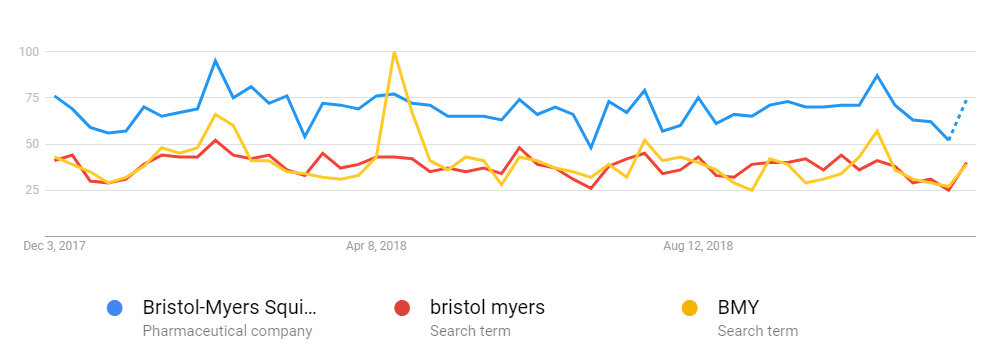
\includegraphics[width=1\textwidth]{fig/bmyStatisticsGoogleTrendsAddedExplanation.png}
 \caption{Google Search Volume for company trend, ticker trend and search term trend for Bristol-Myers Squibb.}
\label{fig:bmyStatisticsGoogleTrends}
\end{figure}
\begin{figure}[h!]
  \centering
    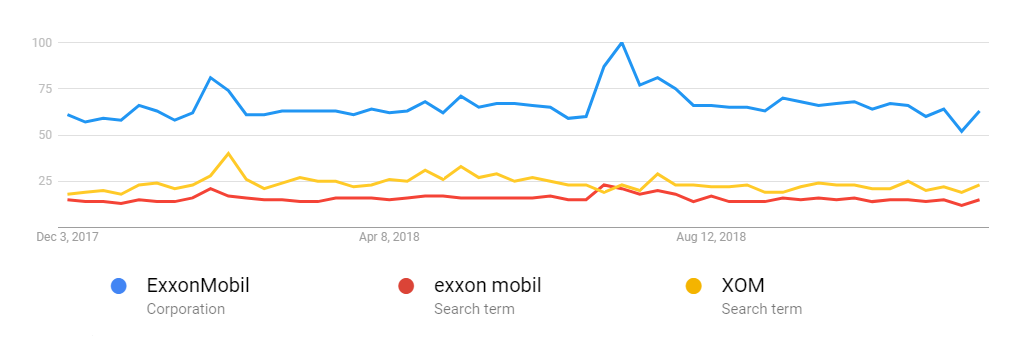
\includegraphics[width=1\textwidth]{fig/xomStatisticsGoogleTrendsAddedExplanation.png}
 \caption{Google Search Volume for company trend, search term trend and ticker trend for Exxon Mobil.}
\label{fig:xomStatisticsGoogleTrends}
\end{figure}

\section{Wikipedia views}

Wikipedia views are collected from Wikipedia Pageviews Analysis which is is a tool to extract pageview volume for individual Wikipedia pages. Pageviews Analysis gives us the absolute view counts on the pages for each of the S\&P 100 companies on a daily, weekly and yearly basis. To get company specific data we map company names to the Wikipedia pages describing them.
\\\\
We use Equation \eqref{log_asvi} to calculate the Abnormal Pageviews Volume ($AbnWiki$) at week $t$, which is basically the same equation as Equation \eqref{abnormal_volume}:
\begin{equation}
   \label{abnormal_pageviews_volume} 
   AbnWiki_{t} = log(Wiki_{t}) - log[Med(Wiki_{t-8},...,Wiki_{t-1})] 
\end{equation}
   where $log(Wiki_{t})$ is the logarithm of the Pageviews Volume at week $t$, and $log[Med(Wiki_{t-8},...,Wiki_{t-1})]$is the logarithm of the median $Wiki$ for the previous 8 weeks.
\section{Monthly variables}
 We also calculate the monthly average for all variables by taking the average over the last 4 weeks. 
\begin{equation}
   \label{monthly_var} 
   variable^{m}_t = avg(variable^{w}_{t},...,variable^{w}_{t-3}) 
\end{equation}
where $m$ and $w$ indicate monthly and weekly variables. The reason to include monthly variables is to capture any long term dependencies between the variables. Instead of including several lagged variables we are using monthly variables to keep the model parsimonious.
\\\\
Finally, all variables, including monthly averages, are normalized to have a standard deviation of one across the pooled data. Normalization makes the coefficients easier to compare across variables and regression models.

\section{Information demand and supply}
We have made a graphical representation of information demand and supply for Microsoft and Google, which can be seen in figure \ref{fig:informationDemandAndSupplyGraphsMicrosoft} and \ref{fig:informationDemandAndSupplyGoogleGraphs} respectively. Information supply is represented by news count, while information demand is represented by Wikipedia, concept trend, search term trend and ticker trend. The search term trend and concept trend graphs fluctuate in the same manner, which indicate that they contain much of the same information. However, ticker trend seems to have different fluctuations compared to search term trend and concept trend. This may be related to that ticker trend measures investor attention, which means people that are looking for information to make financial investments.
\\\\
Furthermore, it is interesting to note that news count seems to lag ticker trend in both figure \ref{fig:informationDemandAndSupplyGraphsMicrosoft} and \ref{fig:informationDemandAndSupplyGoogleGraphs}. Because the variables have different fluctuation patterns and therefore seem to measure different aspects of information demand and supply, it might be valuable to include all the variables in our further analyses. 
\begin{figure}[h!]
  \centering
    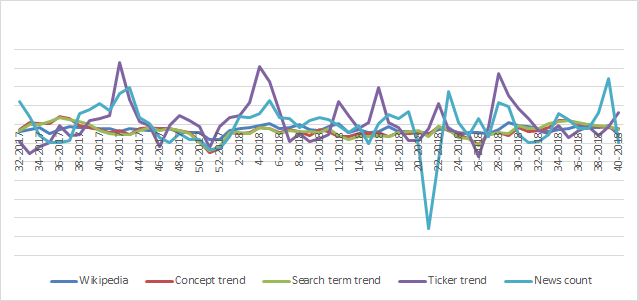
\includegraphics[width=1\textwidth]{fig/informationSupplyAndDemandGraphsMicrosoftWithoutYAxis.png}
 \caption{Information demand and supply for Microsoft. News count is an information supply variable, while concept trend, search term trend, ticker trend and Wikipedia Pageviews are information demand variables.}
\label{fig:informationDemandAndSupplyGraphsMicrosoft}
\end{figure}
\begin{figure}[h!]
  \centering
    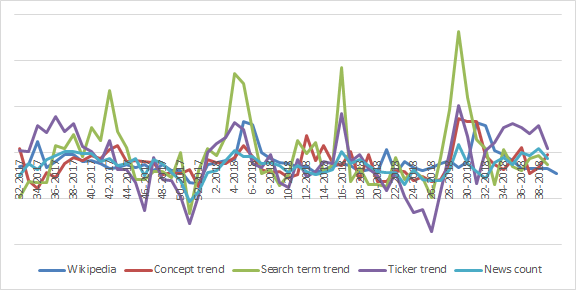
\includegraphics[width=1\textwidth]{fig/informationSupplyAndDemandGraphsGoogleWithoutYAxis.png}
 \caption{Information demand and supply for Google. News count is an information supply variable, while concept trend, search term trend, ticker trend and Wikipedia Pageviews are information demand variables.}
\label{fig:informationDemandAndSupplyGoogleGraphs}
\end{figure}
\begin{table}[!htbp] \centering 
  \caption{Descriptive statistics before st.dev normalization} 
  \label{tab:desc_stat} 
\begin{tabular}{@{\extracolsep{5pt}}lcccccc} 
\\[-1.8ex]\hline 
\hline \\[-1.8ex] 
Statistic & \multicolumn{1}{c}{Mean} & \multicolumn{1}{c}{St. Dev.} & \multicolumn{1}{c}{Min} & \multicolumn{1}{c}{Pctl(25)} & \multicolumn{1}{c}{Pctl(75)} & \multicolumn{1}{c}{Max} \\ 
\hline \\[-1.8ex] 
log\_return & 0.002 & 0.031 & $-$0.209 & $-$0.013 & 0.020 & 0.224 \\ 
w\_vol & 0.010 & 0.004 & 0.003 & 0.007 & 0.012 & 0.049 \\ 
logmedian\_VOLUME & 0.017 & 0.341 & $-$1.307 & $-$0.199 & 0.207 & 1.875 \\ 
logmedian\_news\_count & 0.026 & 0.657 & $-$4.635 & $-$0.305 & 0.335 & 5.513 \\ 
logmedian\_wiki & 0.025 & 0.195 & $-$0.953 & $-$0.061 & 0.075 & 2.629 \\ 
logmedian\_concept\_trend & 0.004 & 0.150 & $-$0.869 & $-$0.053 & 0.047 & 2.813 \\ 
logmedian\_search\_term\_trend & 0.002 & 0.146 & $-$1.030 & $-$0.056 & 0.054 & 1.966 \\ 
logmedian\_ticker\_trend & 0.009 & 0.197 & $-$3.738 & $-$0.056 & 0.054 & 1.833 \\ 
\hline \\[-1.8ex] 
\end{tabular} 
\end{table} 

\clearpage

\subsection*{Stationarity}
% Stationarity test are run from the stationarity_test Jupyter file

To avoid spurious regression it is important that variables are stationary. The log-median transformation described above should remove most non-stationary effects from our time series. Subtracting previous values removes any linear trend, and taking the logarithm minimizes other non-linear relations. 
\\\\
To test for stationarity in the transformed variables we run the argumented Dickey-Fuller (ADF) test for each variable and each company separately. The test indicates stationarity for all variables after normalization, except for volatility. Since volatility, from economic theory and empirical data, is known to be stationary but with high shock persistent, we will treat it as stationary going forwards. 









